\chapter{Исследовательская часть}

\section{Интерфейс приложения}

На рисункaх  \ref{fig:interface} -- \ref{fig:working1} приведено изображение интерфейса главного экрана приложения.
\FloatBarrier
\begin{figure}[h!]
	\centering{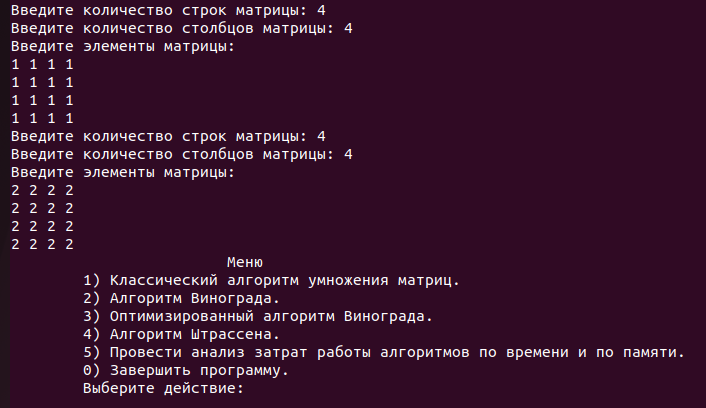
\includegraphics[scale=0.7]{photos/interface.png}}
	\caption{Интерфейс}
	\label{fig:interface}
\end{figure}
\FloatBarrier

На экране приложения пользователь может ввести две матрицы, для которых необходимо вычислить умножение, а также выбрать метод, который будет использован для этого вычисления. 
В результате выводится полученное умножение.
\FloatBarrier
\begin{figure}[h!]
	\centering{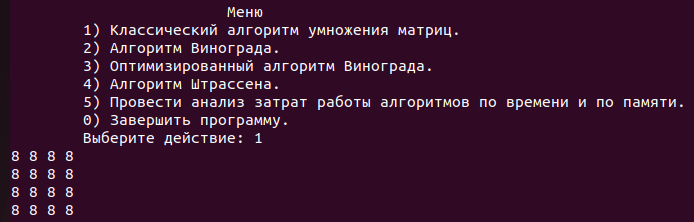
\includegraphics[scale=0.7]{photos/working1.png}}
	\caption{Пример работы стандартного алгоритма умножения матриц}
	\label{fig:working1}
\end{figure}
\FloatBarrier

\section{Технические характеристики}

Технические характеристики устройства, на котором выполнялось тестирование:

\begin{itemize}
	\item операционная система: Ubuntu 22.04.3 LTS;
	\item оперативная память: 12 Гб;
	\item процессор: AMD® Athlon silver 3050u with radeon graphics × 2;
\end{itemize}

\section{Время выполнения реализаций алгоритмов}

Замеры времени работы реализованных алгоритмов проводились для квадратных матриц.
На рисунке 4.3 приведено сравнение реализации всех алгоритмов умножения матриц, которые содержат 2, 4, 8, 16, 32, 64, 128, 256 элементов.
\begin{figure}[ht!]
	\begin{center}
		\captionsetup{singlelinecheck = false, justification=centerfirst}
		\begin{tikzpicture}
			\begin{axis}[
				xlabel={Размер матрицы},
				ylabel={Время в секундах},
				width = 0.95\textwidth,
				height=0.5\textheight,
				xmin=0, xmax=256,
				ymode=log, 
				legend pos=north west,
				legend style={font=\footnotesize},
				xmajorgrids=true,
				grid style=dashed,
				]
				
				\addplot[
				blue,
				semithick,
				mark = *,
				mark size = 3pt,
				thick,
				] file {graph/normal.csv};
				
				\addplot[
				red,
				semithick,
				mark = *,
				] file {graph/vinograd.csv};
				
				\addplot[
				green,
				semithick,
				mark = *,
				] file {graph/opt.csv};
				
				\addplot[
				purple,
				semithick,
				mark = *,
				] file {graph/shtrassen.csv};
				
				\legend{
					Стандартный алгоритм,
					Алгоритм Винограда,
					Оптимизированный алгоритм Винограда,
					Алгоритм Штрассена
				}
			\end{axis}
			
		\end{tikzpicture}
		\centering
		\caption{Сравнение времени работы реализаций алгоритмов}
		\label{fig:graph1}
	\end{center}
	
\end{figure}

\clearpage

\section{Используемая память}

Использование памяти при стандартным алгоритмом теоретически равно: 
\begin{equation}
	\label{eq:normal}
	\begin{aligned}
		3 \cdot sizeof(size\_t) + {n_1} \cdot {m_1} \cdot sizeof(int) + sizeof(vector<vector<int>>) + \\
		+{n_2} \cdot {m_2} \cdot sizeof(int) + sizeof(vector<vector<int>>) + {n_1} \cdot {m_2} \cdot \\ 
		\cdot sizeof(int) + sizeof(vector<vector<int>>),
	\end{aligned}
\end{equation}
где:
\begin{itemize}
	\item $3 \cdot sizeof(size\_t) $ --- хранение количество строк и столбцов первой матрицы и количество столбцов второй матрицы;
	\item ${n_1} \cdot {m_1} \cdot sizeof(int) $ --- хранение количество элементов матрицы;
	\item $sizeof(vector<vector<int>>$ --- структура матрицы.
\end{itemize}

Для обычного и оптимизированного алгоритма Винограда умножения матриц можно посчитать по следуюшей формуле:
\begin{equation}
	\label{eq:vinograd}
	\begin{aligned}
		4 \cdot sizeof(size\_t) + {n_1} \cdot {m_1} \cdot sizeof(int) + \\
		+sizeof(vector<vector<int>>) + {n_2} \cdot {m_2} \cdot sizeof(int) + \\
		+ sizeof(vector<vector<int>>) + {n_1} \cdot {m_2} \cdot sizeof(int) + \\
		+sizeof(vector<vector<int>> + {n_1} \cdot sizeof(int) + {m_2} \cdot sizeof(int)),
	\end{aligned}
\end{equation}
где 
\begin{itemize}
	\item $4 \cdot sizeof(size\_t) $ -- хранение количество строк и столбцов матриц;
	\item ${n_1} \cdot {m_1} \cdot sizeof(int) $ --- хранение количество элементов матрицы;
	\item ${n_1} \cdot sizeof(int) $ --- храниние количество элементов одномерного массива
	\item $sizeof(vector<vector<int>>$ --- структура матрицы.
\end{itemize}

По расходу памяти алгоритм Винограда и оптимизированный алгоритм Винограда проигрывают от стандартного алгоритма умножения матриц. 
Это из-за того, что в алгоритме Винограда и оптимизированном алгоритме Винограда хранятся дополнительные два одномерных массива. 

\begin{figure}[ht!]
	\begin{center}
		\captionsetup{singlelinecheck = false, justification=centerfirst}
		\begin{tikzpicture}
			\begin{axis}[
				xlabel={Размер матрицы},
				ylabel={Память в байтах},
				width = 0.95\textwidth,
				height=0.5\textheight,
				xmin=0, xmax=256,
				ymode=log, 
				legend pos=north west,
				legend style={font=\footnotesize},
				xmajorgrids=true,
				grid style=dashed,
				]
				
				\addplot[
				blue,
				semithick,
				mark = *,
				mark size = 3pt,
				thick,
				] file {graph/normal_mem.csv};
				
				\addplot[
				red,
				semithick,
				mark = *,
				] file {graph/vinograd_mem.csv};
				
				\addplot[
				green,
				semithick,
				mark = *,
				] file {graph/opt_mem.csv};
				
				\addplot[
				purple,
				semithick,
				mark = *,
				] file {graph/shtrassen_mem.csv};
				
				\legend{
					Стандартный алгоритм,
					Алгоритм Винограда,
					Оптимизированный алгоритм Винограда,
					Алгоритм Штрассена
				}
			\end{axis}
			
		\end{tikzpicture}
		\centering
		\caption{Сравнение размеров реализаций алгоритмов в байтах}
		\label{fig:graph2}
	\end{center}
	
\end{figure}

\clearpage

\section*{Вывод}
В данном разделе было произведено сравнение количества затраченного времени и памяти алгоритмов умножения матриц. 
Наименее затратным по времени оказался оптимизированный алгоритм Винограда. 
Получисля такой результат потому, что у него сложность меньше $O(n^{2,3755})$, пока у стандартного алгоритм сложность $O(n^{3})$, а у алгоритма Штрассена $O(n^{\log _{2}7})$.

По памяти наименее затратным оказался стандартный алгоритм умножения матриц, так как он содержить наименьшее количество структуры.


